\documentclass[]{article}
\usepackage{lmodern}
\usepackage{amssymb,amsmath}
\usepackage{ifxetex,ifluatex}
\usepackage{fixltx2e} % provides \textsubscript
\ifnum 0\ifxetex 1\fi\ifluatex 1\fi=0 % if pdftex
  \usepackage[T1]{fontenc}
  \usepackage[utf8]{inputenc}
\else % if luatex or xelatex
  \ifxetex
    \usepackage{mathspec}
    \usepackage{xltxtra,xunicode}
  \else
    \usepackage{fontspec}
  \fi
  \defaultfontfeatures{Mapping=tex-text,Scale=MatchLowercase}
  \newcommand{\euro}{€}
\fi
% use upquote if available, for straight quotes in verbatim environments
\IfFileExists{upquote.sty}{\usepackage{upquote}}{}
% use microtype if available
\IfFileExists{microtype.sty}{%
\usepackage{microtype}
\UseMicrotypeSet[protrusion]{basicmath} % disable protrusion for tt fonts
}{}
\usepackage[margin=1in]{geometry}
\usepackage{longtable,booktabs}
\usepackage{graphicx}
\makeatletter
\def\maxwidth{\ifdim\Gin@nat@width>\linewidth\linewidth\else\Gin@nat@width\fi}
\def\maxheight{\ifdim\Gin@nat@height>\textheight\textheight\else\Gin@nat@height\fi}
\makeatother
% Scale images if necessary, so that they will not overflow the page
% margins by default, and it is still possible to overwrite the defaults
% using explicit options in \includegraphics[width, height, ...]{}
\setkeys{Gin}{width=\maxwidth,height=\maxheight,keepaspectratio}
\ifxetex
  \usepackage[setpagesize=false, % page size defined by xetex
              unicode=false, % unicode breaks when used with xetex
              xetex]{hyperref}
\else
  \usepackage[unicode=true]{hyperref}
\fi
\hypersetup{breaklinks=true,
            bookmarks=true,
            pdfauthor={Julian Jenkins III, Vivian Chow, Lisa Blaskey, Emily Kuschner, Saba Qasmieh, Leah Gaetz, J. Christopher Edgar, Pratik Mukherjee, Randall Buckner, Srikantan S. Nagarajan, Wendy K. Chung, John E. Spiro, Elliott H. Sherr, Jeffrey I. Berman, Timothy P.L. Roberts},
            pdftitle={Auditory Evoked M100 Response Latency is Delayed in Children with 16p11.2 Deletion but not 16p11.2 Duplication},
            colorlinks=true,
            citecolor=blue,
            urlcolor=blue,
            linkcolor=magenta,
            pdfborder={0 0 0}}
\urlstyle{same}  % don't use monospace font for urls
\setlength{\parindent}{0pt}
\setlength{\parskip}{6pt plus 2pt minus 1pt}
\setlength{\emergencystretch}{3em}  % prevent overfull lines
\setcounter{secnumdepth}{0}

%%% Use protect on footnotes to avoid problems with footnotes in titles
\let\rmarkdownfootnote\footnote%
\def\footnote{\protect\rmarkdownfootnote}

%%% Change title format to be more compact
\usepackage{titling}

% Create subtitle command for use in maketitle
\newcommand{\subtitle}[1]{
  \posttitle{
    \begin{center}\large#1\end{center}
    }
}

\setlength{\droptitle}{-2em}
  \title{Auditory Evoked M100 Response Latency is Delayed in Children with
16p11.2 Deletion but not 16p11.2 Duplication}
  \pretitle{\vspace{\droptitle}\centering\huge}
  \posttitle{\par}
  \author{Julian Jenkins III, Vivian Chow, Lisa Blaskey, Emily Kuschner, Saba
Qasmieh, Leah Gaetz, J. Christopher Edgar, Pratik Mukherjee, Randall
Buckner, Srikantan S. Nagarajan, Wendy K. Chung, John E. Spiro, Elliott
H. Sherr, Jeffrey I. Berman, Timothy P.L. Roberts}
  \preauthor{\centering\large\emph}
  \postauthor{\par}
  \predate{\centering\large\emph}
  \postdate{\par}
  \date{July 6, 2015}



\begin{document}

\maketitle


{
\hypersetup{linkcolor=black}
\setcounter{tocdepth}{2}
\tableofcontents
}
\section{Abstract}\label{abstract}

Individuals with the 16p11.2 BP4-BP5 copy number variant (CNV) exhibit a
range of behavioral phenotypes that that may include mild impairment in
cognition and clinical diagnoses of Autism Spectrum Disorder (ASD). To
better understand auditory processing impairments in populations with
this chromosomal variation, auditory evoked responses were examined in
children with the 16p11.2 deletion, 16p11.2 duplication and age-matched
controls. Stimuli consisted of sinusoidal binaural tones presented
passively while children underwent recording with magnetoencephalography
(MEG). The primary indicator of auditory processing impairment was the
latency of the \textasciitilde{}100ms ``M100'' auditory response
detected by MEG, with the 16p11.2 deletion population exhibiting
profoundly delayed M100 latencies relative to controls. This delay
remained even after controlling for potential confounds such as age and
cognitive ability. No significant difference in M100 latency was
observed between 16p11.2 duplication carriers and controls.
Additionally, children meeting diagnostic criteria for ASD (16p11.2
deletion carriers) exhibited non-significant latency delays when
compared to the corresponding CNV carriers not meeting criteria for ASD.
Present results indicate that 16p11.2 deletion is associated with
auditory processing delays analogous to (but substantially more
pronounced than) those previously reported in ``idiopathic'' ASD.

\begin{center}\rule{0.5\linewidth}{\linethickness}\end{center}

\section{Introduction}\label{introduction}

Individuals with the deletion and duplication of the BP4-BP5 16p11.2
locus (chr16: 29.5-30.1 Mb) have varied behavioral phenotypes, including
Autism Spectrum Disorder (ASD) (Hanson et al. 2010; Qureshi et al.
2014), language impairment (Hanson et al. 2010; Shinawi et al. 2010;
Zufferey et al. 2012) and developmental delays. Individuals with the
16p11.2 deletion and duplication, particularly duplication carriers, can
also have a phenotype ``within normal range'' although they still tend
to demonstrate significant impairments compared with family members who
do not carry the deletion or duplication. Mouse models and human data
demonstrate that the consequences of deletion of the 16p11.2 CNV may be
more severe than the duplication (Horev et al. 2011; Stefansson et al.
2014). The mechanistic linkage between this copy number variant (CNV)
and behavioral/clinical/diagnostic findings, however, remains elusive.

Studies have shown delayed auditory evoked neuromagnetic field
components (M100: Roberts et al. 2010; M50: Roberts et al. 2013) in
conditions such as autism spectrum disorder (ASD). Delayed evoked
responses persist after variance associated with cognitive function (IQ)
and language ability is considered. It has been speculated that delays
in early auditory processing may reveal atypical development of auditory
sensory cortex and/or thalamocortical connections (Roberts et al. 2009,
2013) and may functionally underlie subsequent higher order neuronal
dysfunction, leading to observed behavioral sequelae.

The purpose of this study is to assess the left and right superior
temporal gyrus (STG) auditory evoked neuromagnetic field M100 component,
detected by magneto-encephalography (MEG), in children with the 16p11.2
deletion and duplication in comparison to age-matched controls.
Specifically, we test the hypothesis that STG M100 latency will be
delayed in the genetically-defined cohorts, in particular the deletion
carriers. A hypothesis is that genes or other conserved elements in the
16p11.2 interval are necessary for generation of an age-appropriate M100
response (for example, by coding for synapse formation), and that, as
with other CNVs, deletion carriers will be more severely impacted than
duplication carriers. An alternative hypothesis predicts that the M100
response, as an indicator of atypical functional activity, more closely
ties to phenotype and might thus be atypical in both deletion and
duplication carriers with the same neurocognitive phenotype.
Secondarily, given that the 16p11.2 deletion and duplication carriers
share common breakpoints, it might be expected that observed measurement
variability in the M100 will be reduced compared to measures in
idiopathic (no known genetic, or other, etiology) ASD populations
(Bijlsma et al. 2009). On the other hand, the variable clinical
phenotypes associated with the 16p11.2 deletion and duplication
(e.g.~heterogeneous expression of ASD diagnosis, language impairment,
and other phenotypes, ranging from mildly to severely impaired) might be
expected to be associated with increased measurement variance of
neuronal indices such as the M100.

A two-center multisite approach was adopted, as part of the broader
Simons Variation in Individuals Project (Simons VIP;
\url{http://sfari.org/resources/simons-vip}). The analysis examined the
left and right STG auditory cortex M100 latencies in response to 200,
300, 500 and 1000 Hz sinusoidal tones. These analyses compared 16p11.2
deletions and duplications to age-matched controls and secondarily
explored M100 latencies in the subset of 16p11.2 deletion and
duplication carriers with ASD. We observe that children with the 16p11.2
deletion exhibit M100 delays relative to age-matched controls, of even
greater magnitude than previously reported in idiopathic ASD compared to
age-matched controls. Children with the 16p11.2 duplication exhibit M100
latencies not significantly different from age-matched controls. Meeting
diagnostic criteria for ASD in 16p11.2 CNV probands does not
significantly further prolong latency.

\section{Materials and Methods}\label{materials-and-methods}

\subsection{Genetic status confirmation and neuropsychological
assessment}\label{genetic-status-confirmation-and-neuropsychological-assessment}

16p11.2 deletion and duplication pediatric participants included
individuals with the same recurrent \textasciitilde{}600kb deletion
(chr16:29,652,999 - 30,199,351; hg19) without other pathogenic CNVs or
known genetic diagnoses (Zufferey et al. 2012). Probands with the
16p11.2 deletion and duplication were identified through routine
clinical chromosome microarrays and recruited through the Simons VIP
Connect website to participate (Simons VIP Consortium 2012). Cascade
genetic testing of family members using whole genome high-resolution
oligonucleotide arrays (Agilent 244k, G4411B, Agilent Technologies, Palo
Alto, CA) determined if the deletion or duplication was de novo or
inherited, to determine if carriers had other clinically significant
CNVs (which would be exclusionary) and to identify other 16p11.2 CNV
carriers within the family (Baldwin et al. 2008). Age-matched controls
underwent chromosome microarrays to rule out pathological CNVs at the
16p11.2 locus and throughout the genome. Eight (out of 35) 16p11.2
deletion participants and three (out of 16) 16p11.2 duplication
participants met criteria for ASD as established by clinical impression
using DSM-IV-TR criteria (American Psychiatric Association 2000).

Following screening, families participated in initial data collection at
one of four Simons VIP phenotyping sites (Boston Children's Hospital,
Baylor College of Medicine, University of Washington, Children's
Hospital of Philadelphia) for a comprehensive and standardized multi-day
evaluation. The study was approved by the Institutional Review Board at
each participating institution; all participants provided informed
consent prior to data collection. All diagnostic interviewing and
cognitive testing was videotaped for later review. Standardization of
measurements across sites included mandatory formalized, standardized
training on all measures through in-person training sessions and
webinars for all clinicians, cross-site reliability and maintenance
through monthly clinician conference calls and periodic videotape
review, and validation and diagnostic confirmation through data review
and observation of video recorded sessions by independent consultants.

Experienced, licensed clinicians gave best-estimate, clinical DSM-IV-TR
diagnoses using all information obtained during the research evaluation.
Information was based on the standardized interview, questionnaire, and
observation processes described below as well as results from
standardized administration of the Diagnostic Interview Schedule for
Children (Shaffer et al. 2000), SCL-90 (Derogatis 1977) and review of
available medical records and prior testing. To capture the range of
psychiatric presentation, exclusionary criteria for diagnoses were not
considered (e.g., if a child met criteria for ADHD and ASD, both
diagnoses were considered). Autism-specific diagnostic measures included
the Autism Diagnostic Observation Scale (Lord et al. 2000) and the
Autism Diagnostic Interview -- Revised (Rutter et al. 2003); both
measures were administered by research-reliable clinicians.

Participants were administered cognitive measures by experienced and
licensed child psychologists via the standardization procedure described
above. The Social Responsiveness Scale was used as a continuous measure
of social and behavioral problems with high scores thought to correspond
with greater likelihood of ASD (Constantino and Gruber 2005). Cognitive
and language measures included: Differential Abilities Scale, Second
Edition (Elliott 2007), Wechsler Abbreviated Scales of Intelligence
(Wechsler 2003), the Clinical Evaluation of Language Fundamentals,
Fourth Edition (Semel et al. 2003), Comprehensive Test of Phonological
Processing- Nonword Repetition subtest (Wagner et al. 1999). Standard
scores were used, or when standard scores were not available, ratio
intelligence quotient (IQ) scores were calculated, for Full Scale IQ
(FSIQ), Verbal IQ (VIQ), and Nonverbal IQ (NVIQ). Control exclusion
criteria included known neurologic or psychiatric diagnosis in the
participant or any sibling, English as a second language, drug use or
incidental findings on MRI.

Based on geographical proximity, participants proceeded to MEG
evaluation at one of two sites (Children's Hospital of Philadelphia, or
University of California, San Francisco).

\subsection{Participants}\label{participants}

One hundred thirty-seven child participants (Children's Hospital of
Philadelphia (CHOP): 63, University of California, San Francisco (UCSF):
74) were recruited (46 16p11.2 deletions, 25 duplications, 66 controls).
Of this initial pool, 19 were excluded based on eligibility criteria
(e.g., psychological/neurological profile, drug use, incidental findings
from MRI). Of the residual pool of 118, who underwent MEG, 19 were found
inevaluable due primarily to motion artifact (6 controls, 7 deletions, 6
duplications). Thus, of the evaluable 99 participants (CHOP: 47, UCSF:
52) forty-eight were age-matched controls, thirty-five 16p11.2 deletion
carriers and sixteen 16p11.2 duplication carriers. Of the age-matched
controls there were nineteen females and twenty-nine males, with five
left-handed, thirty-five right-handed and eight ambidextrous (Oldfield
1971). Of the 16p11.2 deletion carriers there were fifteen females and
twenty males, with nine left-handed, twenty-two right-handed and four
ambidextrous. Of the 16p11.2 duplication carriers, there were six
females and ten males, with thirteen right-handed and three
ambidextrous.

\subsection{Stimuli, procedure and
delivery}\label{stimuli-procedure-and-delivery}

200 Hz, 300 Hz, 500 Hz and 1000 Hz sinusoidal tones were passively
presented. Tones were generated with LabView, sampled at 44.1 kHz with
16-bit resolution and were of 400 ms duration with 10 ms linear onset
and offset ramps. Prior to data acquisition, an auditory threshold test
was conducted with 1000 Hz tones of 300 ms duration and 10 ms rise time,
binaurally presented (starting at a comfortable hearing level) and
decreased until reaching auditory threshold for each ear. The
experimental tones were presented 45 dB above threshold, with each tone
presented 130 times. After completion of MEG scanning, structural MRIs
were acquired using a 1mm isotropic ME-MP-RAGE 3D T1 sequence (Siemens
Trio™ 3T, Siemens Medical Solutions, Erlangen, Germany).

Experimental stimuli were presented using an Edirol UA-1x external
D-to-A converter using E-Prime stimulus presentation software. Stimuli
were delivered binaurally through a TDT SA1 power amp, a pair of PA5
attenuators and a MA5 microphone amplifier to Eartone ER3A transducers
and non-magnetic air tubes and eartip inserts. The ISI varied
pseudo-randomly in the range 900 to 1100 ms.

\subsection{MEG recording}\label{meg-recording}

Data were acquired using either a 275-channel whole-head magnetometer
(CHOP) or a 272-channel whole-head magnetometer (UCSF). Using
anti-aliasing filters, recording bandwidth was DC-300 Hz, sampled at
1200 Hz/channel. Prior to scanning and data acquisition, three
head-position indicator coils attached to the participant's scalp at
nasion and left and right pre-auricular points provided continuous
information on head position and orientation relative to the MEG
sensors. Electrodes attached to the left and right clavicles and to the
bipolar oblique (upper and lower left sites) recorded electrocardiogram
(ECG) and electro-oculogram (EOG).

\subsection{MEG analysis}\label{meg-analysis}

Source space analyses were implemented using BESA 5.2 (BESA Research,
Gräfelfing, Germany). Prior to evoked response analysis (offline
averaging, filtering and baseline correction), the data were downsampled
to 500 Hz with a zero-phase high-pass filter (cutoff frequency: 166.7
Hz, -24dB/octave slope). Eyeblink and heart artifact correction was
implemented as described in Roberts et al. (2010). Epochs with artifacts
other than blinks and heartbeats were rejected on the basis of amplitude
and gradient criteria (amplitude \textgreater{} 1200fT/cm, gradients
\textgreater{} 800fT/cm/sample). For each condition (i.e., 200, 300,
500, and 1000 Hz tones), epochs from the continuous recording were
defined 500 ms pre- and post-trigger onset.

The presence of a M100 response in the left and right STG was determined
using a standard dipole source model that transformed the averaged and
filtered MEG sensor data into brain space (MEG data co-registered to the
Montreal Neurologic Institute (MNI) averaged brain) using a dipole model
with multiple sources (Scherg and von Cramon 1985; Scherg 1990; Scherg
and Berg 1996). Specifically, the source model included left and right
STG regional sources positioned at Heschl's gyrus and nine fixed
regional sources modeling brain background activity and acting as probe
sources for additional activity. Each participant's eye-blink and
heartbeat source vectors were included in the individual source models
(Lins et al. 1993; Berg and Scherg 1994).

Auditory evoked responses were analyzed after applying three Butterworth
filters: (i) a 1 Hz forward-phase high-pass (-6dB/octave slope); (ii) a
zero-phase 40Hz low-pass filter (-48dB/octave slope) and (iii) a 60 Hz
notch filter (5 Hz width). For each tone, the evoked response was
baseline corrected over the pre-trigger interval. M100 latency peak for
the left and right STG dipoles was determined based on identification of
an M100 in the sensor and source waveforms within an acceptable range
(85-185 ms), resemblance to canonical M100 magnetic field topography and
dipole goodness of fit (GOF). Adjustments (extensions) to the acceptable
latency range were considered based on the age of the participants
(younger participants typically have longer latencies; see Roberts et
al. 2010; Roberts et al., 2013; Edgar et al. 2013). If a participant did
not exhibit an auditory cortex magnetic field topography for a given
condition, those observations were excluded from further analysis.
Typically, the M100 either followed a detectable M50 or preceded a
detectable M200 (or both). A total of nineteen participants (two
controls, seventeen deletions; four meeting ASD criteria) in the age
range 7.98 -- 12.60 years had the M100 search latency window extended.

\subsection{Statistical analysis}\label{statistical-analysis}

Statistical analyses were performed using R 3.1.2 (R Core Team 2014). A
given result was considered significant for (i) \emph{p} \textless{}
0.05 (linear mixed models, Wald Type II Chi-square tests, correlation
tests, Tukey HSD) and (ii) z \textgreater{} 2 (z-statistic, Tukey HSD).
Results were visualized using the \texttt{ggplot2} package (Wickham
2009).

Linear mixed models (LMMs) with a dependent variable of M100 latency
(ms) were performed with random effect of Subject, fixed effects of Case
(16p11.2 deletion vs.~16p11.2 duplication vs.~neurotypical control),
Hemisphere, Stimulus Condition (200, 300, 500, 1000 Hz) and Acquisition
Site (CHOP vs.~UCSF) with subject Age as a covariate and random slopes
of Stimulus Condition and Hemisphere. LMMs were fit via maximum
likelihood using the \texttt{lme4} package (Bates et al. 2014).
Significance of the fixed effects was assessed using Wald Type II
Chi-square tests via the \texttt{car} package (Fox and Weisberg 2011)
and multiple comparisons, significance of individual factor levels and
effect sizes were assessed using Tukey HSD via the `multcomp' package
(Hothorn et al. 2008). The primary model evaluated was a main effects
model of
\texttt{Hemisphere\ +\ Stimulus\ Condition\ +\ Case\ +\ Age\ +\ Site\ +\ (Stimulus\ Condition\ +\ Hemisphere\ \textbar{}\ Subject)}.
Additional models with NVIQ and VIQ as a covariate were also assessed.
Correlation tests (Spearman's rho) between neuropsychological assessment
scores (VIQ, NVIQ, SRS total score, CTOPP non-word repetition) and M100
latency were assessed in 16p11.2 deletion and duplication carriers.
Comparisons of 16p11.2 deletion and duplication carriers meeting vs.~not
meeting ASD diagnostic criteria were assessed using a LMM of Hemisphere
+ Stimulus Condition + ASD status + Age + Site; random effects
structures were the same as in previous analyses.

\section{Results}\label{results}

\subsection{M100 recording success
rate}\label{m100-recording-success-rate}

No significant difference in sensation level was observed between groups
with mean differences \textless{}5dB (\(\chi\)\textsuperscript{2} =
3.810, df = 2, \emph{p} = 0.148). For the participants not rejected from
analysis on the grounds of excessive motion, evaluable auditory evoked
responses from at least one stimulus condition (tone frequency x
hemisphere) were obtained in all 35 of the participants with the 16p11.2
deletion and all 16 participants with the 16p11.2 duplication. In
age-matched controls evaluable data was obtained in 45 out of 48
participants. In terms of success eliciting at least one evaluable M100
response component, there was no significant difference between groups,
even considering motion-based rejection: controls: 45/54; deletions:
35/42; duplications: 16/22, \(\chi\)\textsuperscript{2} = 1.33 \emph{p}
= 0.51. Not all subjects had 8 evaluable responses (left, right
hemisphere, 4 stimulus conditions). 266 evaluable responses (out of 384
possible) were observed in controls (69.3\%), 203 (out of 280 possible)
were observed in 16p11.2 deletion carriers (72.5\%) and 65 (out of 128
possible) were observed in 16p11.2 duplications (50.8\%). Analysis of
deviance on the per-stimulus success rates indicated the success rate
for 16p11.2 duplication carriers was, however, less than that of 16p11.2
deletion carriers (estimate = 0.281, SE = 0.222, z = -4.231, \emph{p}
\textless{} 1e-04) or age-matched controls (estimate = 0.314, SE =
0.209, z = -3.748, \emph{p} \textless{} 0.001). Success rates for
16p11.2 deletion carriers vs.~age-matched controls did not differ
(estimate = 0.539, SE = 0.174, z = 0.902, \emph{p} = 0.637). Summaries
of age and psychological score distributions for participants with
evaluable data are shown in Table 1.

\textbf{\emph{Table 1.}} Summary of age and psychological score
distributions for each case: participants with evaluable M100 data.
Values are means ± one standard deviation. For participants with
evaluable M100 data (i.e., at least one observed M100 out of eight
measurements) there was a significant difference in the age
distributions (\emph{F}(2, 93) = 3.88, \emph{p} = 0.024) between cases;
this was due to the mean age of the controls being higher than the
population mean (estimate = 0.776, SE = 0.279, t = 2.781, \emph{p} =
0.017). However, the age distributions of each population overlapped
within their mean + 1 SD of each other, indicating the distributions
were comparable. Age was nevertheless considered as a covariate in all
analyses. There were also significant differences in the NVIQ
(\emph{F}(2, 89) = 22.96, \emph{p} = 9.103e-09), VIQ (\emph{F}(2, 89) =
20.59, \emph{p} = 4.485e-08), CELF-4 (\emph{F}(2, 82) = 34.92, \emph{p}
= 1.068e-11), SRS (\emph{F}(2, 84) = 43.97, \emph{p} = 5.235e-14) and
CTOPP (\emph{F}(2,84) = 24.464, \emph{p} = 4.245e-09) distributions.

\begin{longtable}[c]{@{}llll@{}}
\toprule
--- & Age-matched controls & 16p11.2 deletion carriers & 16p11.2
duplication carriers\tabularnewline
\midrule
\endhead
Age range (years) & 7.31 - 17.15 & 7.98 - 17.03 & 7.38 -
16.92\tabularnewline
Mean age (years) & 12.82±2.56 & 11.32±.2.65 & 11.45±2.41\tabularnewline
N (evaluable) & 45 & 35 & 16\tabularnewline
NVIQ & 105.73±11.88 & 90.09±15.07 & 83.06±10.68\tabularnewline
VIQ & 107.24±13.72 & 85.37±17.05 & 91.69±14.09\tabularnewline
CELF-4 & 106.22±11.22 & 75.81±20.80 & 84.62±13.18\tabularnewline
SRS & 16.68±11.89 & 71.51±34.38 & 72.06±41.22\tabularnewline
CTOPP nonword repetition & 9.23±1.95 & 5.64±2.64 &
7.64±1.45\tabularnewline
\bottomrule
\end{longtable}

\subsection{M100 latency effects}\label{m100-latency-effects}

Figure 1 illustrates a typical auditory evoked response from
representative individuals in the control, 16p11.2 deletion and 16p11.2
duplication groups using the FieldTrip package (Oostenveld et al. 2011).
Note that whereas source modeled waveform morphology is similar across
participants, the latency of the peak ``M100'' evoked response differs,
later in the 16p11.2 deletion (compared to control) and similar in the
16p11.2 duplication (compared to control).

\begin{figure}[htbp]
\centering
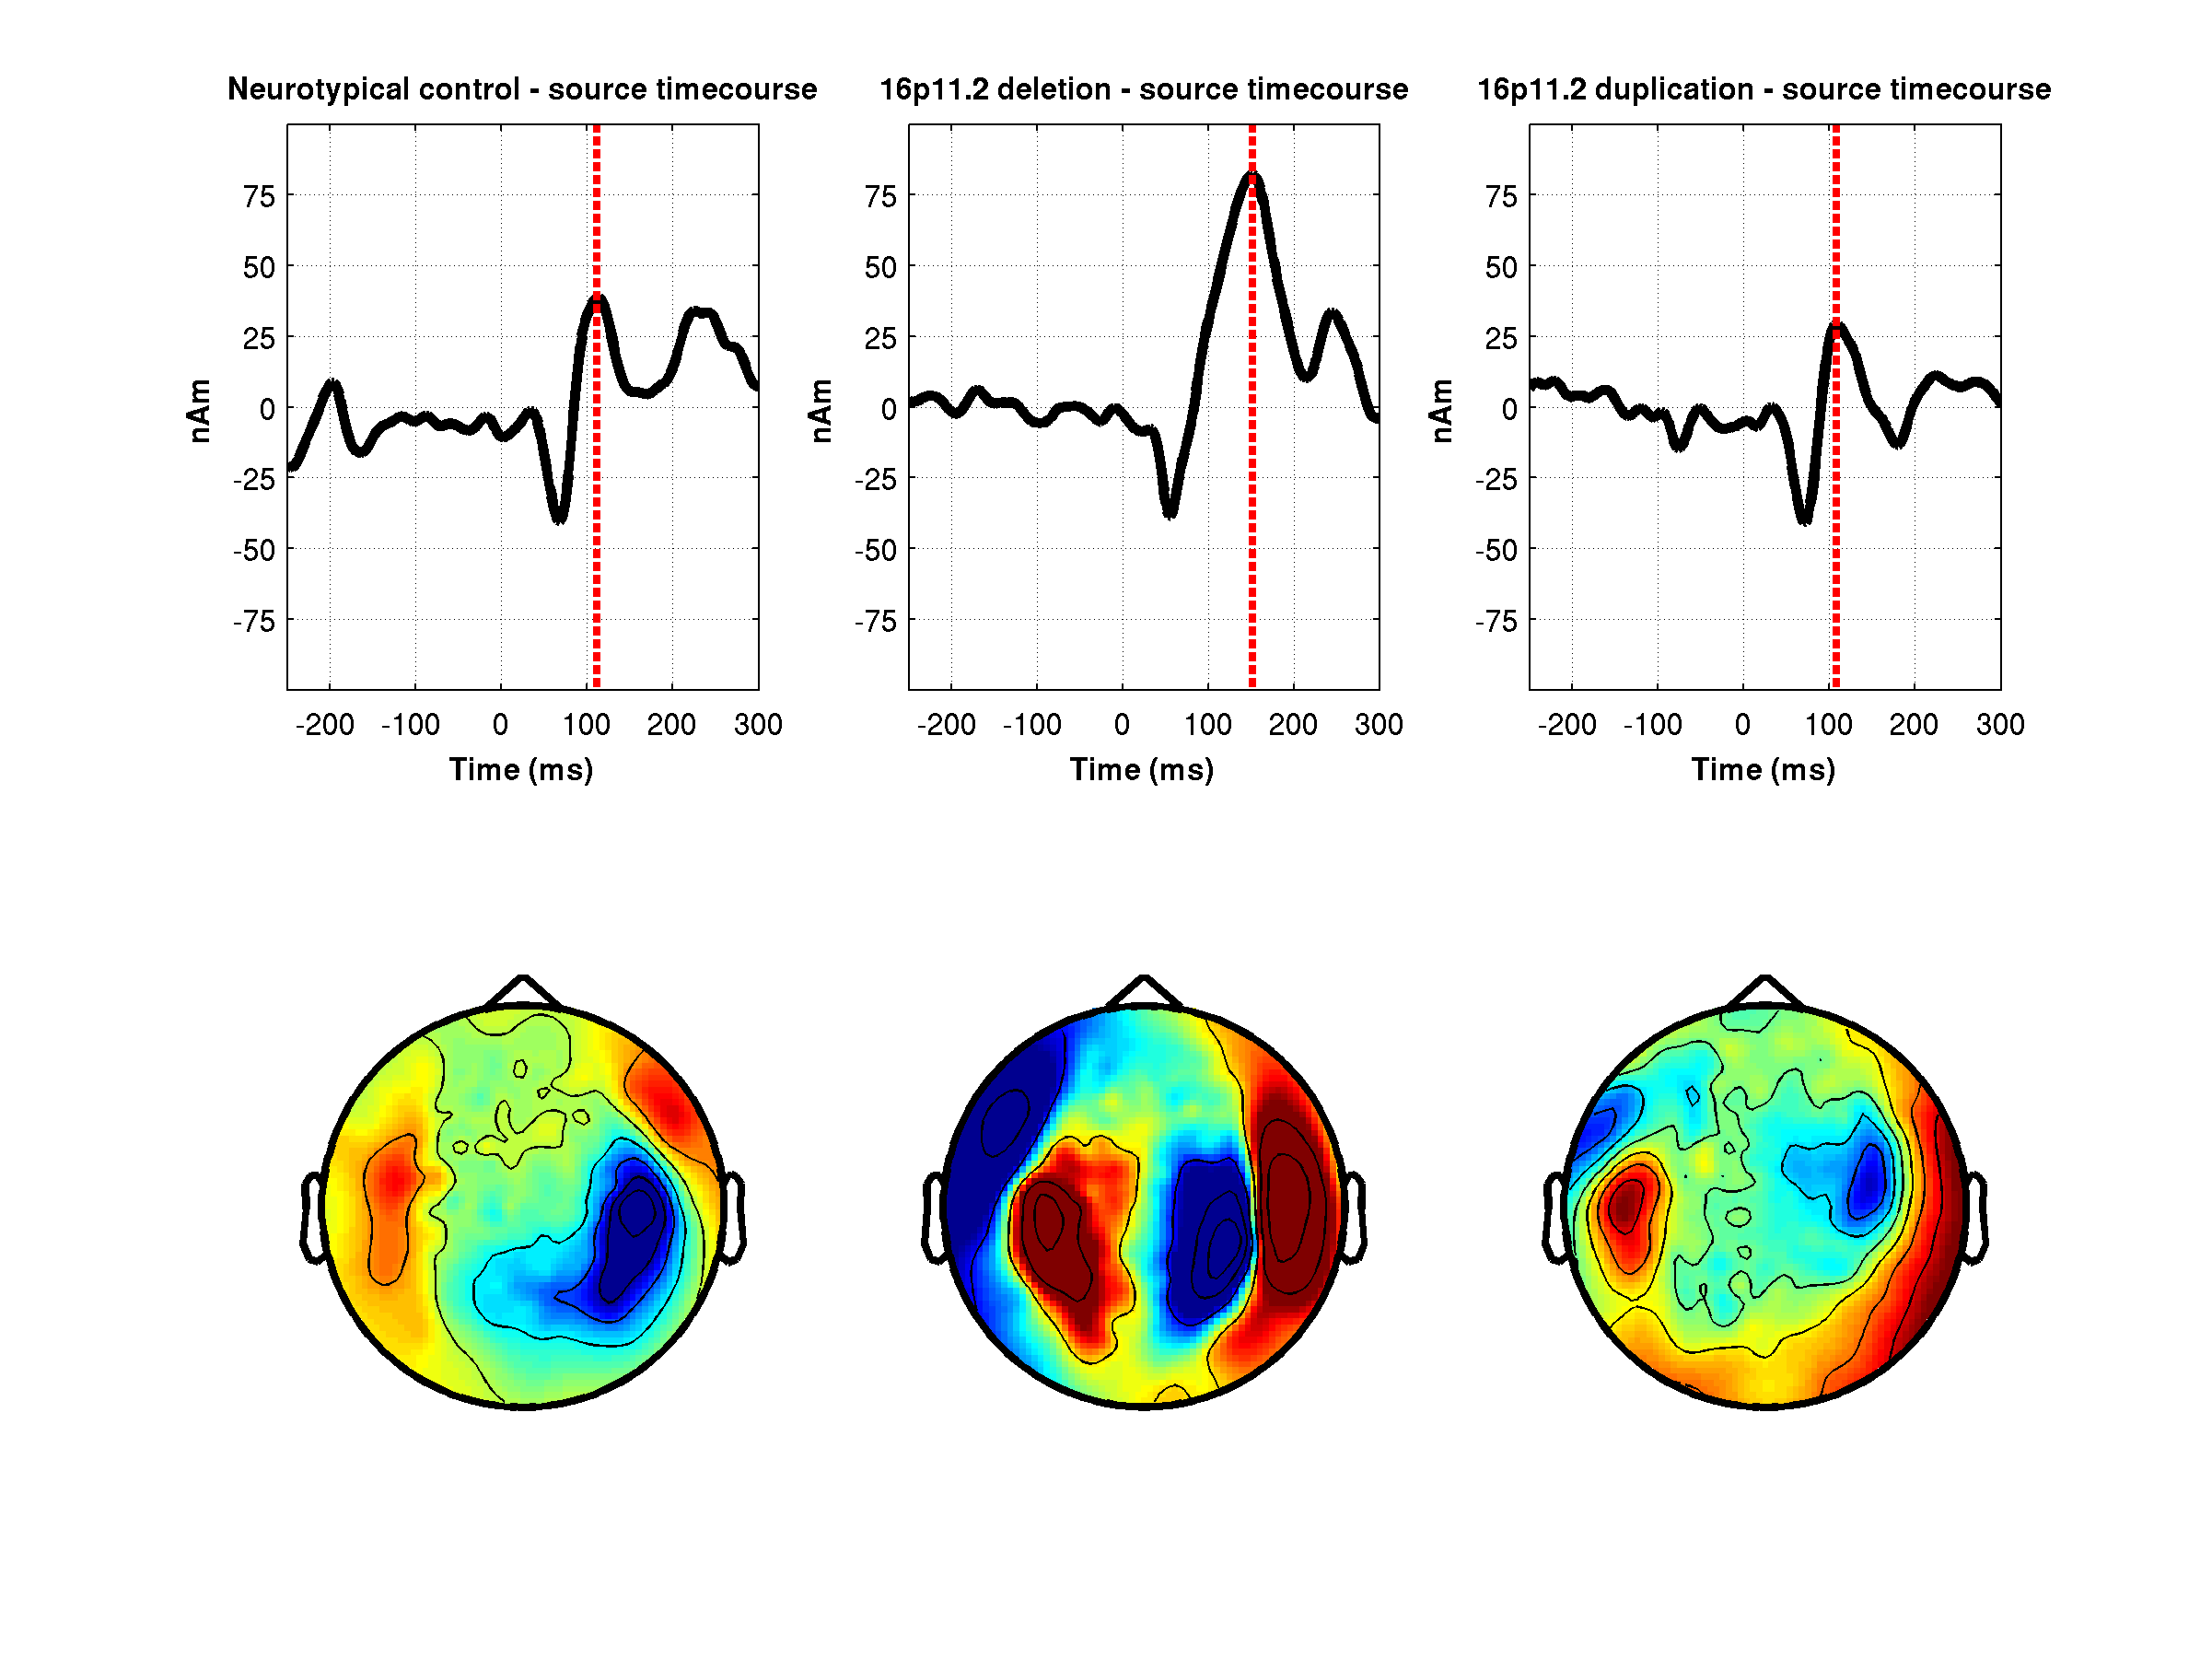
\includegraphics{figure-1-updated-final.png}
\caption{Representative control, 16p11.2 deletion and 16p11.2
duplication auditory response profiles. Artifact-corrected source
waveforms to a 1000 Hz tone in the RH for a control (left column; 11.78
y.o.), 16p11.2 deletion carrier (middle column; 9.62 y.o.) and 16p11.2
duplication carrier (right column; 13.98 y.o.). All participants are
within 1 SD of the mean population age. Source timecourses are in the
top row and source-sink distribution in the bottom row (source = red,
sink = blue). M100 latency for the 16p11.2 deletion carrier is 152ms,
for the control is 112ms and for the 16p11.2 duplication carrier is
108ms. From the visualization, the M100 peak is clearly seen based on
the magnetic field deflections and the canonical source-sink
distribution; there is more lateralization present in the control and as
such, the corresponding LH source-sink distribution is not displayed.}
\end{figure}

Within each group, M100 latency was negatively associated with age
(decreasing latency with increasing age), as has been shown before
(Paetau et al. 1995; Roberts et al. 2009; Edgar et al. 2014). Figure 2a
shows associations between M100 latency vs.~age for each group. Although
regression slopes do not differ (-3.9±0.8 ms/yr control vs -5.6±1.5ms/yr
16p11.2 deletion vs -2.4±1.4 ms/yr 16p11.2 duplication; \emph{F}(2, 93)
= 1.197, \emph{p} = 0.307), there is a clear shift between the
regression lines, indicating a longer latency in the 16p11.2 deletion
group and suggesting a earlier, although non-significant, latency
(\textasciitilde{}5ms) in 16p11.2 duplications vs.~controls. Whereas the
regression lines in Fig 2a reflect an effective M100 latency derived
from the responses from both hemispheres to individual tones of four
different frequencies, the robust persistence of the general trend of
significantly increased latency in deletion carriers is shown in Figs.
2b and c, breaking down fixed effects of stimulus frequency (Fig 2b) and
hemisphere (Fig 2c). For each stimulus type and for both hemispheres,
the observed group differences between controls, 16p11.2 deletion and
duplication carriers are recapitulated. Case differences are further
explained in Table 2.

\begin{figure}[htbp]
\centering
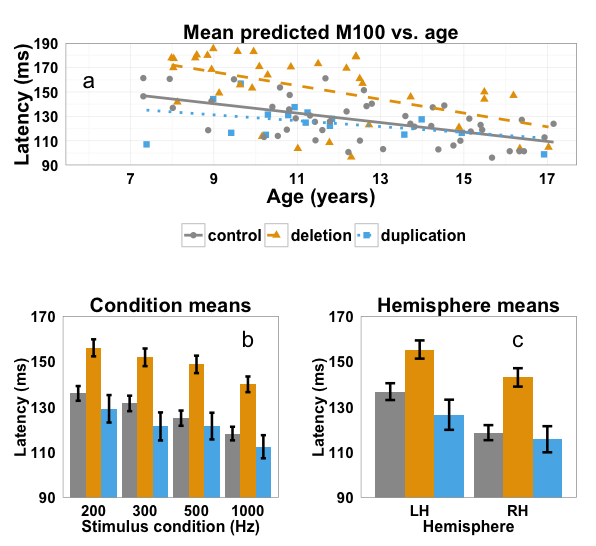
\includegraphics{figure-2-resubmssion.png}
\caption{Latency vs.~age regression, stimulus condition and hemispheric
means for each case. Age-matched controls are delineated in gray circles
with a solid outline, 16p11.2 deletion carriers by orange triangles with
a dashed outline, 16p11.2 duplication carriers by light blue squares
with a dotted outline. (a) For all three cases, there is an inverse
relationship between M100 latency (across stimulus conditions and
hemispheres) and age, with the slopes between the cases not
significantly different (\emph{F}(2, 93) = 1.197, p = 0.307). (b) M100
latency for each case and stimulus condition. For each stimulus
condition, 16p11.2 deletion carriers exhibit a delay in M100 latency
relative to age-matched controls, while 16p11.2 duplication carrier
latencies are not significantly different. (c) As with the mean M100
latencies in (a) and for each stimulus condition (b), similar patterns
of M100 latency delay are present in 16p11.2 deletion carriers for each
hemisphere.}
\end{figure}

\textbf{\emph{Table 2.}} Least-squares means for age-matched controls,
16p11.2 deletion and 16p11.2 duplication carriers: overall (modeling
factors of Hemisphere, Stimulus Condition, Case, Site and covarying with
Age) and within each hemisphere (modeling Stimulus Condition, Case, Site
and covarying with Age), 16p11.2 deletion carriers exhibit an
approximately 21 ms delay in M100 compared to age-matched controls. The
difference between 16p11.2 deletion carriers and controls was
significant overall and in each hemisphere (LH: estimate = 18.4ms, SE =
5.5, z = 3.339, \emph{p} = 0.002; RH: estimate = 23.4ms, SE = 5.5, z =
4.293, \emph{p} \textless{} 0.001).

\begin{longtable}[c]{@{}llll@{}}
\toprule
Mean & Age-matched controls & 16p11.2 deletion carriers & 16p11.2
duplication carriers\tabularnewline
\midrule
\endhead
Overall (ms) & 127.2±3.1 & 149.0±3.6 & 120.9±5.3\tabularnewline
LH (ms) & 136.7±3.7 & 155.3±4.0 & 126.5±6.6\tabularnewline
RH (ms) & 118.6±3.3 & 143.0±4.1 & 115.7±5.8\tabularnewline
\bottomrule
\end{longtable}

Age-covaried LMM indicated significant main effects for Hemisphere (L vs
R; \(\chi\)\textsuperscript{2} = 40.477, df = 1, \emph{p} = 1.990e-10),
Stimulus Condition (200 vs 300 vs 500 vs 1000Hz;
\(\chi\)\textsuperscript{2} = 162.930, df = 3, \emph{p} \textless{}
2.2e-16) and Case (16p11.2 deletion vs.~16p11.2 duplication vs.~control;
\(\chi\)\textsuperscript{2} = 32.265, df = 2, \emph{p} = 9.857e-08). In
particular, responses were earlier in the right than left STG (estimate
= -14.6ms, SE = 2.3, z = -6.362, \emph{p} = 1.990e-10) and earlier to
higher frequencies (500 and 1000 Hz) than lower frequencies (min.
estimate = -4.3ms, SE = 1.1, z = -4.047, \emph{p} \textless{} 0.001).

Whereas 16p11.2 deletion M100 latencies were longer than age-matched
controls (estimate = 20.9ms, SE = 4.3, z = 4.822, \emph{p} \textless{}
1e-04), responses in 16p11.2 duplication carriers were not different
from controls, although their mean M100 latency value was slightly
earlier (estimate = -5.4ms, SE = 5.6, z = -0.978, \emph{p} = 0.588).
There was no effect of sex (\(\chi\)\textsuperscript{2} = 0.198, df = 1,
\emph{p} = 0.657). No effect of nonverbal IQ (NVIQ) or verbal IQ (VIQ)
as a covariate was observed (NVIQ: \(\chi\)\textsuperscript{2} = 0.334,
df = 1, \emph{p} = 0.563; VIQ: \(\chi\)\textsuperscript{2} = 0.281, df =
1, \emph{p} = 0.596). There was no effect of recording site (CHOP
vs.~UCSF; \(\chi\)\textsuperscript{2} = 1.484, df = 1, \emph{p} =
0.223). The slight latency difference (5.4ms; 4.4 SE) is likely
attributed to technical or population sampling differences (and site was
nonetheless included in all analyses as a fixed effect). Effect sizes
and Tukey HSD are summarized Table 3.

\textbf{\emph{Table 3.}} Effect size estimate and Tukey HSD for M100
latency between each Case. 16p11.2 deletion carriers exhibit delayed
latencies relative to age-matched controls and 16p11.2 duplication
carriers, while latency differences between 16p11.2 duplication carriers
and age-matched controls are not significantly different, although the
distributions are significantly shifted towards shorter latency for
16p11.2 duplication carriers.

\begin{longtable}[c]{@{}lrrrrr@{}}
\toprule
lhs & rhs & estimate & se & t & p\tabularnewline
\midrule
\endhead
deletion - control & 0 & 20.943815 & 4.343121 & 4.8222961 &
0.0000037\tabularnewline
duplication - control & 0 & -5.448478 & 5.569807 & -0.9782167 &
0.5878473\tabularnewline
duplication - deletion & 0 & -26.392292 & 5.636830 & -4.6821162 &
0.0000069\tabularnewline
\bottomrule
\end{longtable}

Figure 3 summarizes the effect of group, showing least-squares mean M100
latencies (after modeling fixed effects of hemisphere, condition,
acquisition site and covarying age and accounting for individual subject
differences in hemispheric processing and response to the stimulus
conditions as random effects). A pronounced prolongation of M100 latency
is observed in the 16p11.2 deletion group. There is no difference in
mean M100 latency between 16p11.2 duplication carriers and age-matched
controls. M100 latency distribution curves for each population (Fig 3b)
shows that the distributions do, however, differ significantly
(Kolmogorov-Smirnov: min. D = 0.512, \emph{p} = 2.578e-12), with the
16p11.2 duplication cohort shifted towards earlier latencies. Hence the
approximately 5ms earlier latency observed in the 16p11.2 duplication
group mean may indeed represent a non-significant trend, with
statistical significance likely not achieved because of the combination
of small effect size, high variance and low sample number in this cohort
(evaluable n = 16). A power calculation estimate using a difference in
means of 5.4ms, a pooled SD of 7.78ms and requiring 80\% power at an
alpha level of 0.05, suggests an evaluable sample size of at least 33
would be required to resolve group differences between the 16p11.2
duplication and control groups. Nonetheless, our interpretation of the
mean and distribution data is that of a non-significant trend,
unresolvable in the present study.

\begin{figure}[htbp]
\centering
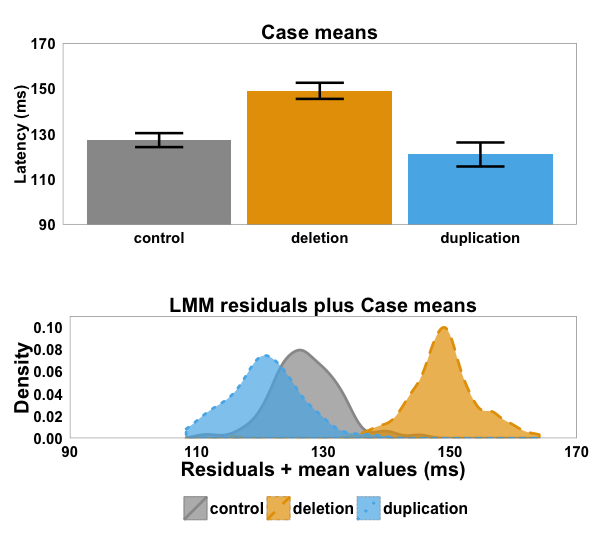
\includegraphics{figure-3-resubmission.png}
\caption{M100 least-squares means and LMM residuals separated by case
means. (a) Least-squares means ± one standard error derived from main
effects model of Hemisphere + Stimulus Condition + Case + Age + Site +
(Stimulus Condition + Hemisphere \textbar{} Subject). Coloring and line
conventions are the same as in Figure 2. (a) Case means illustrate (i)
the large delay exhibited by 16p11.2 deletion carriers
(\textasciitilde{}21ms) and (ii) that 16p11.2 duplication carrier
latency means are not significantly different from controls. (b) Kernel
density estimates (Gaussian window, 512 points, bandwidth calculated
using Silverman's rule of thumb) of residuals plus case means for each
case. This visualization demonstrates (i) the separation of 16p11.2
deletion M100 latencies from controls and (ii) the similar residual
variance in all sub-populations. A Brown-Forsythe test for homogeneity
of variance did not yield a significant difference in residual variance
between each of the populations (\emph{F}(2, 531) = 0.192, \emph{p} =
0.825) but Kolmogorov-Smirnov tests on these distributions indicated the
distributions were significantly different (min. D = 0.512, \emph{p} =
2.578e-12), suggesting that the apparent shift towards a shorter latency
in 16p11.2 duplication carriers represents a trend rendered
non-significant by sample size.}
\end{figure}

Prior reports have indicated a delay in M100 latency as a characteristic
of ASD and a high prevalence of ASD in individuals with the 16p11.2
deletion and duplication. In this sample, 8 out of the 35 evaluable
(22.9\%) 16p11.2 deletion carriers met diagnostic criteria for ASD; 3 of
the 16 evaluable (18.8\%) individuals with 16p11.2 duplications met ASD
criteria. These proportions did not, however, significantly differ
(\(\chi\)\textsuperscript{2} = 0.110, \emph{p} = 0.741). Within the
deletion cohort, comparison of individuals with and without ASD revealed
a non-significant 8ms latency prolongation associated with ASD (estimate
= 8.3ms, SE = 7.0, z = 0.191, \emph{p} = 0.740). The ASD sample size of
3 prohibits statistical analysis within the 16p11.2 duplication cohort.

For each group, collapsing across individuals with and without ASD,
association between least-squares mean M100 latency and the following
psychological scores were examined for NVIQ, SRS, CELF-4 core language
index and CTOPP non-word repetition subtest. Analyses revealed no within
group associations (min. S = 9285.475, \(/rho\) = 0.248, \emph{p} =
0.114), but confirmed overall latency prolongation in the 16p11.2
deletion group.

\section{Discussion}\label{discussion}

The main result of this study is a pronounced (\textasciitilde{}20ms)
delay in the latency of the M100 component of the auditory evoked
response in children with the 16p11.2 BP4-BP5 deletion. There was no
significant difference in M100 latency in 16p11.2 duplications
vs.~controls. Main effects of stimulus type and hemisphere were
observed, along with the dependency of M100 with age, consistent with
previous reports. Of note, the overall effect of (\textasciitilde{}20\%)
increased M100 latency in 16p11.2 deletion carriers transcended each of
these factors.

However, the observed non-significant shortening of latency in 16p11.2
duplications (as opposed to prolongation in 16p11.2 deletions) is not
inconsistent with other gene-dosage opposing effects that have been
reported. For example, 16p11.2 gene dosage has opposing effects on head
circumference, with macrocephaly in 16p11.2 deletion carriers and
microcephaly in 16p11.2 duplication carriers (Shinawi et al. 2010),
opposing effects on brain volume by structural MRI (Qureshi et al. 2014)
and opposing effects on microstructure assessed by diffusion MRI (Owen
et al. 2014). A speculative interpretation is that one or more genes in
the 16p11.2 region may be necessary to ensure a ``typical'' M100;
haploinsufficiency of such genes or conserved elements may lead to a
delayed M100 evoked response; excess dosage of such genetic material may
have no additional impact, or may lead to a slight facilitation of the
M100 evoked response component (with the degree of facilitation limited
and of modest amount). This hypothesis, which requires further
investigation, nonetheless offers a putative biological mechanism
linking genetic and neurophysiological differences.

Additionally there was no significant difference in M100 latency between
16p11.2 deletion carriers who met (vs.~not meeting) ASD diagnostic
criteria. We speculate that the additional, although non-significant,
latency prolongation associated with ASD diagnosis may arise from
additional distinct and additive factors acting within the setting of
16p11.2 CNV sensitization, perhaps akin to those factors observed in
idiopathic ASD. Previous studies have hypothesized biophysical
mechanisms underlying M100 latency delays associated with maturation of
thalamocortical white matter pathways or synaptic transmission. Genetic
contributions to these mechanisms as well as association between
atypical development in ASD and these mechanisms remain to be
elucidated.

A limitation, and topic for further exploration, was the difference in
evaluable data success rates between groups (lower in the 16p11.2
duplication group). Data were rendered non-evaluable primarily for
reasons of compliance (movement) and low signal-to-noise ratio. Not only
does this point to intrinsic differences between the groups, but it also
limits our interpretation to the subset of 16p11.2 duplication carriers
with evaluable data, and thus constitutes a form of potential
ascertainment bias.

The lack of association between M100 latency and the
clinical/behavioral/neuro-psychological measures (i.e., NVIQ, SRS,
CELF-4 and CTOPP), along with the distinct difference in M100 latency
between 16p11.2 deletion and duplication carriers (despite
clinical/behavioral deficits in both groups) suggests that M100 latency
is not directly predictive of clinical/behavioral outcome. Rather, as
discussed above, the influence of 16p11.2 copy number on M100 latency
offers a speculative link between genetics and neurophysiology, perhaps
partially bridging the chasm of gene to behavior. Although not
explicitly tested in this study, it is notable that the M100 latency
residual distributions (after considering effects of age, stimulus,
hemisphere, case and site) have a standard deviation of the order of
\textasciitilde{}5.6ms, quite similar to that previously observed in
typical controls and idiopathic ASD, and thus reflecting a similar
degree of variability. This suggests, provocatively, that reducing
genetic heterogeneity (at least to the extent achievable by considering
a common CNV) has little effect on the variability of the
neurophysiologic phenotype.

In summary, deletion of the 16p11.2 BP4-BP5 region had a profound effect
on M100 latency with mean delays of approximately 20ms. Duplication of
the same region showed no significant difference in M100 latency. The
influence of ASD diagnosis on M100 latency was marginal and
non-significant. No association between M100 latency and
clinical/behavioral/neuropsychological assessments was observed.
Overall, results provide support for a gene-neurophysiology association
with an observable gene-dosage effect, and implicate the 16p11.2 BP4-BP5
locus as involved in auditory evoked M100 response component generation.

\end{document}
